% 174-23(174쪽) — 한 변의 길이가 3인 정사각형을 9등분 해 중앙의 정사각형을 버린 1회 시행 뒤의 모습(색칠한 정사각형 8개).
% 스캔 그림이 흐려 TikZ 로 다시 그렸다. 라벨은 원문에 있는 3 만 두고 남은 넓이(답)는 적지 않는다.
% 격자는 step= 을 쓰면 시작 모서리 선이 빠지므로 \foreach 로 직접 긋는다.
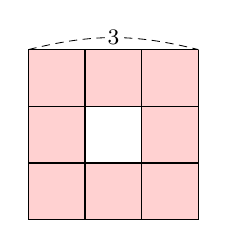
\begin{tikzpicture}[scale=0.72, line width=0.5pt]
  \fill[red!18] (0,0) rectangle (3,3);
  \fill[white] (1,1) rectangle (2,2);
  \foreach \i in {0,1,2,3} {
    \draw (\i,0) -- (\i,3);
    \draw (0,\i) -- (3,\i);
  }
  \draw[densely dashed, line width=0.3pt] (0,3)
    to[bend left=14] node[midway, fill=white, inner sep=1pt, font=\footnotesize] {$3$} (3,3);
\end{tikzpicture}
